\documentclass[11pt,a4paper]{article}

\usepackage[margin=1in]{geometry}
\usepackage{amsmath,amssymb}
\usepackage{graphicx}
\usepackage{booktabs}
\usepackage{float}
\usepackage{xcolor}
\usepackage{hyperref}
\usepackage{listings}
\usepackage{caption}

\hypersetup{
    colorlinks=true,
    linkcolor=blue,
    urlcolor=blue,
    citecolor=blue
}

\lstset{
    language=Python,
    basicstyle=\ttfamily\small,
    keywordstyle=\color{blue},
    commentstyle=\color{gray},
    stringstyle=\color{teal},
    numbers=left,
    numberstyle=\tiny\color{gray},
    stepnumber=1,
    numbersep=8pt,
    breaklines=true,
    frame=single,
    tabsize=4,
    showstringspaces=false
}

\title{HomeWork 07: Random Numbers, Monte Carlo Methods, and Empirical Distributions}
\author{Student Solution}
\date{\today}

\begin{document}
\maketitle

\section{Coin Tosses and the Law of Large Numbers}

\subsection*{Method}
Generate $N=100000$ independent fair coin tosses.  I encode heads as $1$ and tails as $0$.  The running fraction of heads after $n$ tosses is
\begin{equation}
    \hat p_n = \frac{1}{n}\sum_{i=1}^n X_i,
\end{equation}
where $X_i=1$ for heads and $X_i=0$ for tails.  Since the coin is fair, $\mathbb{E}[X_i]=0.5$.  By the Law of Large Numbers,
\begin{equation}
    \hat p_n \longrightarrow 0.5
    \qquad \text{as } n\to\infty.
\end{equation}

\subsection*{Numerical output}
\begin{table}[H]
\centering
\caption{Running fraction of heads for selected values of $n$.}
\begin{tabular}{rcc}
\toprule
$n$ & Running fraction of heads & Deviation from $0.5$ \\
\midrule
10 & 0.700000 & +0.200000 \\
100 & 0.520000 & +0.020000 \\
1,000 & 0.508000 & +0.008000 \\
10,000 & 0.503500 & +0.003500 \\
100,000 & 0.498740 & -0.001260 \\
\bottomrule
\end{tabular}
\end{table}

\begin{figure}[H]
\centering
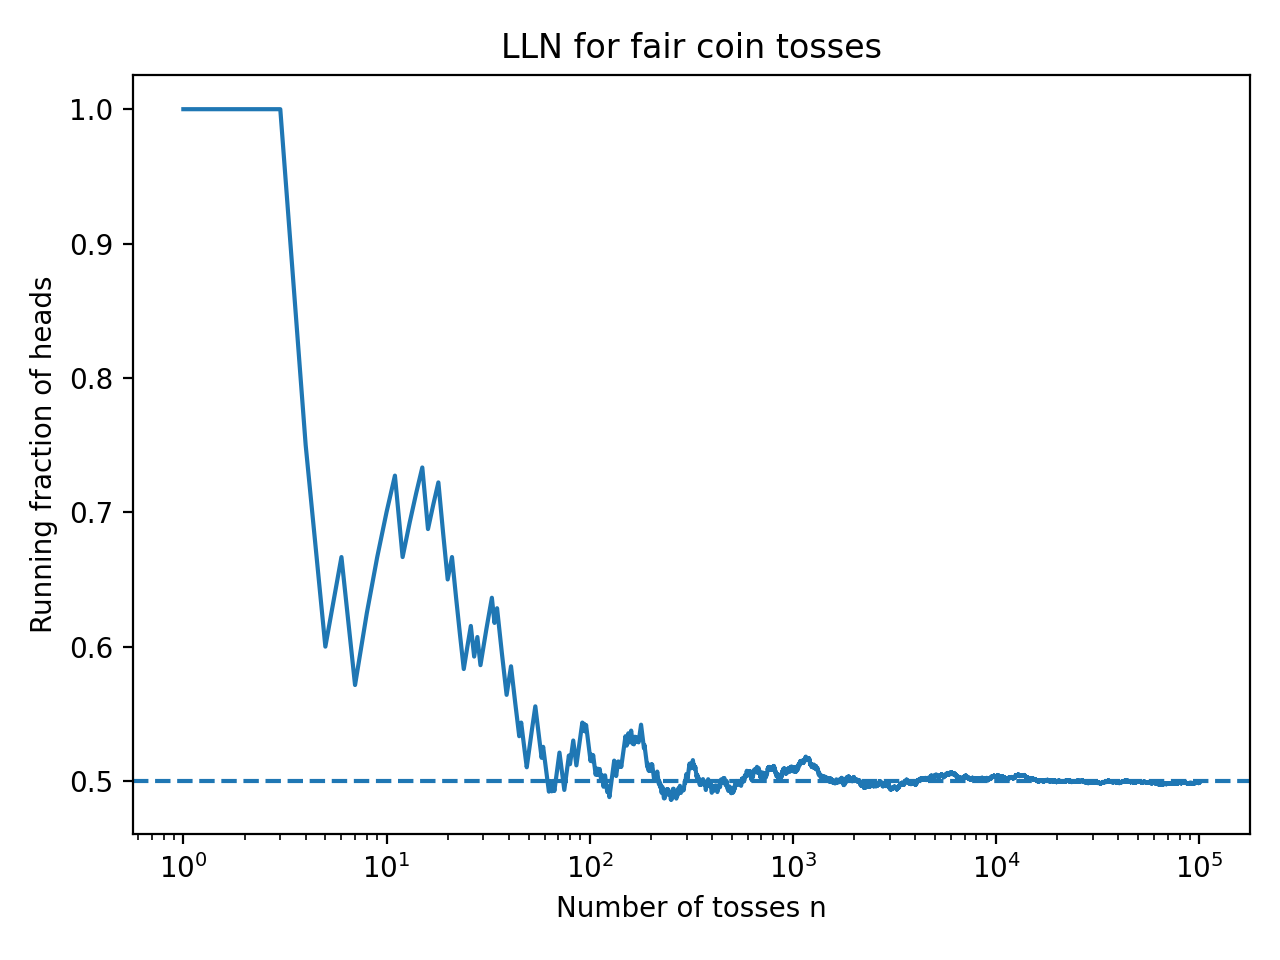
\includegraphics[width=0.78\textwidth]{ex1_coin_lln.png}
\caption{Running fraction of heads.  The dashed line is the theoretical probability $0.5$.}
\end{figure}

For small $n$, the running fraction fluctuates strongly.  As $n$ increases, the fraction becomes increasingly stable and approaches $0.5$.  This is exactly the behavior predicted by the Law of Large Numbers.

\section{Monte Carlo Estimate of $\pi$}

\subsection*{Method}
To estimate $\pi$, generate independent random points $(X,Y)$ uniformly in the unit square $[0,1]^2$.  The probability that a point falls inside the quarter unit circle is
\begin{equation}
    \mathbb{P}(X^2+Y^2\leq 1) = \frac{\pi}{4}.
\end{equation}
Therefore, if $N_{\mathrm{in}}$ is the number of points inside the quarter circle, the Monte Carlo estimator is
\begin{equation}
    \hat\pi_N = 4\frac{N_{\mathrm{in}}}{N}.
\end{equation}
Two independent random number generator streams are used: one for the $x$-coordinates and one for the $y$-coordinates.

\subsection*{Numerical output}
\begin{table}[H]
\centering
\caption{Monte Carlo estimates of $\pi$ for several sample sizes.}
\begin{tabular}{rccc}
\toprule
$N$ & $N_{\mathrm{in}}$ & $\hat\pi_N$ & $|\hat\pi_N-\pi|$ \\
\midrule
100 & 81 & 3.24000000 & 0.09840735 \\
1,000 & 814 & 3.25600000 & 0.11440735 \\
10,000 & 7,802 & 3.12080000 & 0.02079265 \\
100,000 & 78,703 & 3.14812000 & 0.00652735 \\
1,000,000 & 785,752 & 3.14300800 & 0.00141535 \\
\bottomrule
\end{tabular}
\end{table}

\begin{figure}[H]
\centering
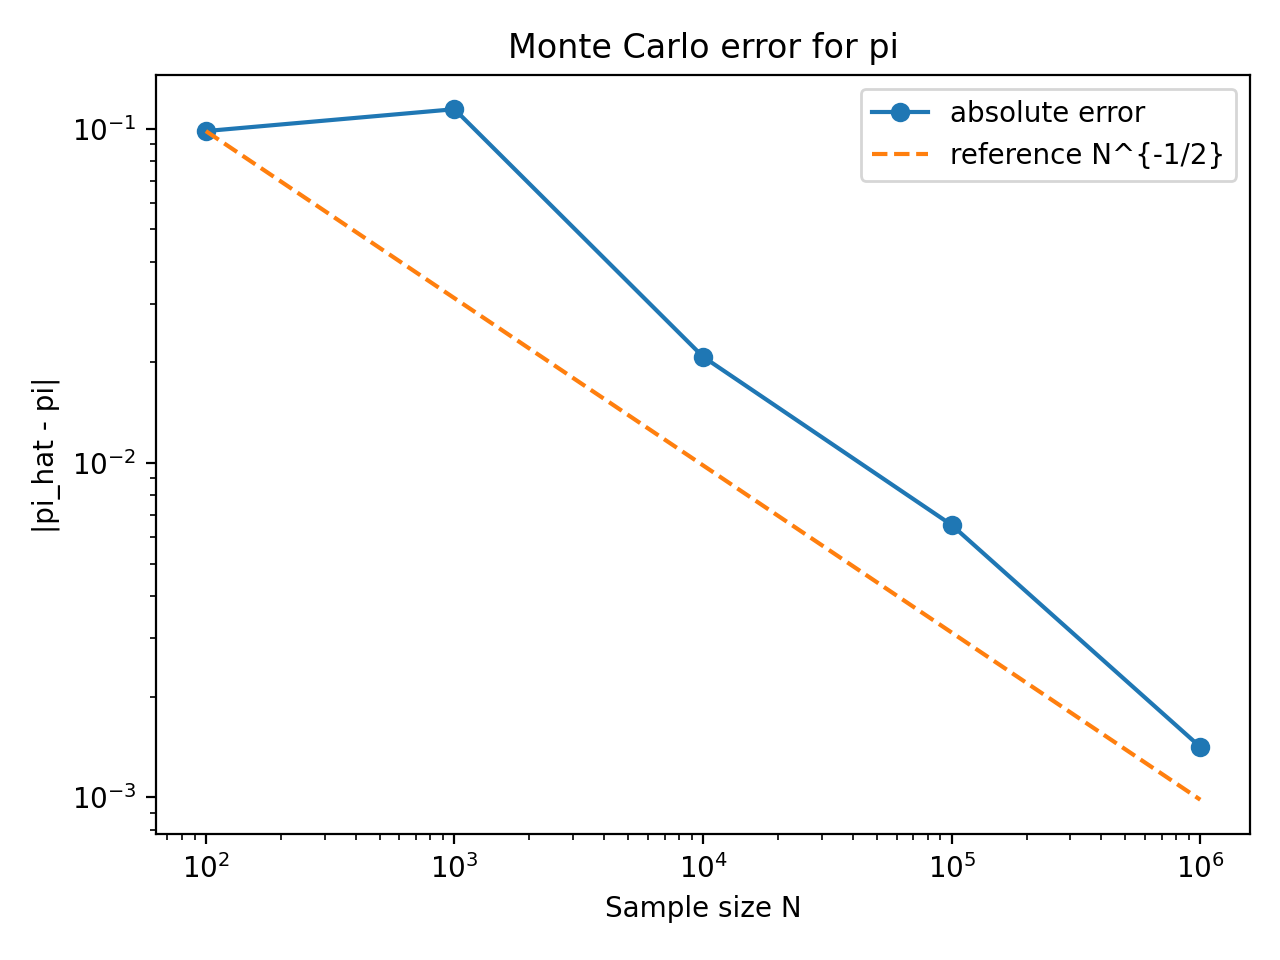
\includegraphics[width=0.78\textwidth]{ex2_pi_error.png}
\caption{Absolute error of the Monte Carlo estimate of $\pi$.  The dashed reference curve is proportional to $N^{-1/2}$.}
\end{figure}

The error does not decrease monotonically at every single sample size because the method is random.  However, its typical magnitude decreases as $N$ grows.  The log-log plot is consistent with the standard Monte Carlo scaling
\begin{equation}
    |\hat\pi_N-\pi| = O(N^{-1/2}).
\end{equation}

\section{Change of Variables: $Y=U^2$}

\subsection*{Analytic density}
Let
\begin{equation}
    U\sim \mathrm{Uniform}(0,1), \qquad Y=U^2.
\end{equation}
For $0<y<1$, the inverse transformation is
\begin{equation}
    u = \sqrt{y}.
\end{equation}
Since $f_U(u)=1$ on $(0,1)$, the density of $Y$ is
\begin{equation}
    f_Y(y) = f_U(\sqrt{y})\left|\frac{d}{dy}\sqrt{y}\right|
           = \frac{1}{2\sqrt{y}},
    \qquad 0<y<1.
\end{equation}

\subsection*{Simulation result}
\begin{figure}[H]
\centering
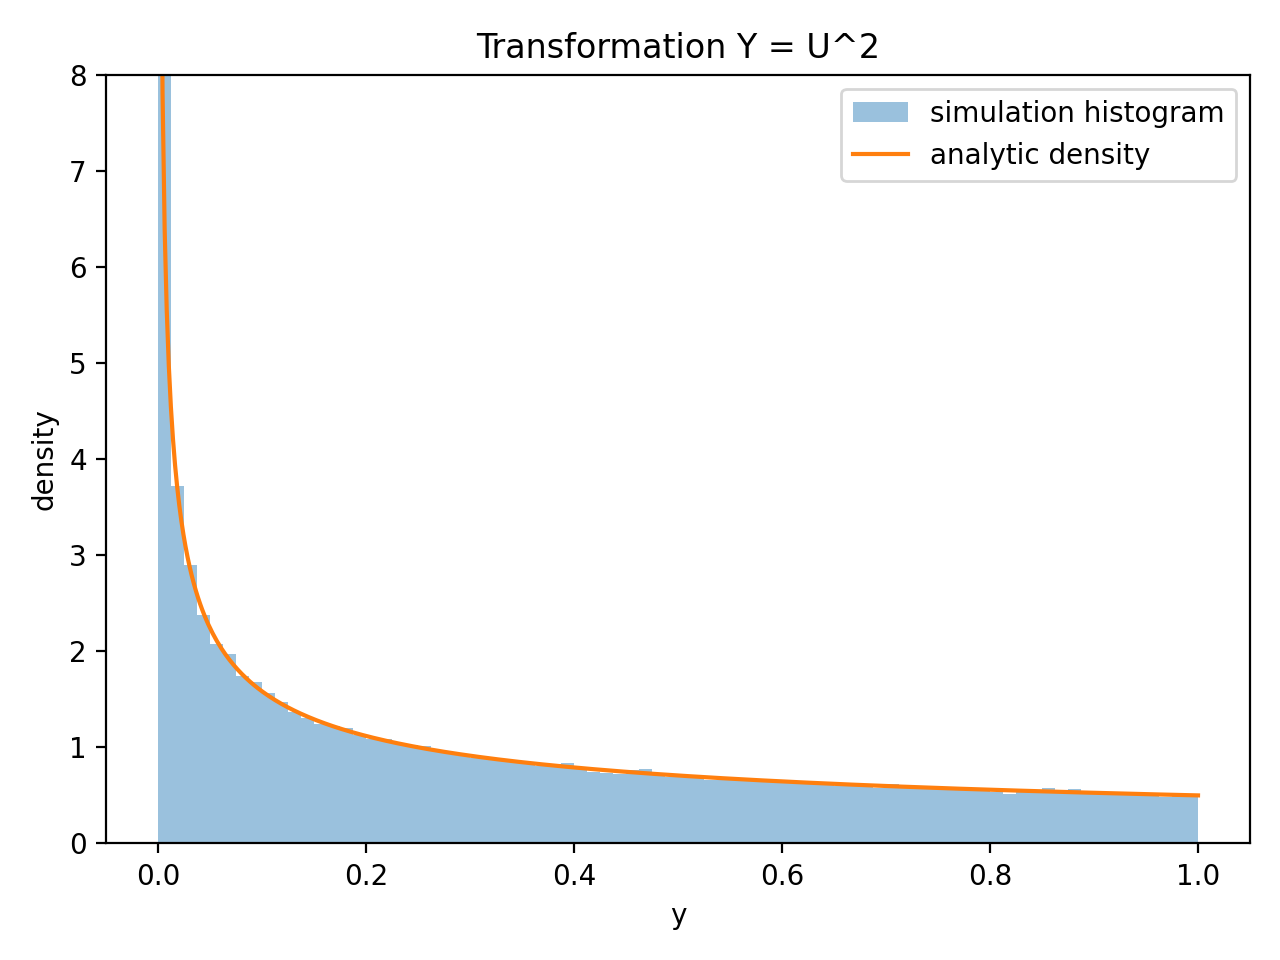
\includegraphics[width=0.78\textwidth]{ex3_y_equals_u2.png}
\caption{Histogram of $Y=U^2$ compared with the analytic density $f_Y(y)=1/(2\sqrt{y})$.}
\end{figure}

The histogram is high near $y=0$ and decreases as $y$ increases.  This agrees with the analytic density $1/(2\sqrt{y})$, which has an integrable singularity at $y=0$.

\section{Inverse Transform Sampling for the Exponential Distribution}

\subsection*{Method}
For an exponential random variable with rate $\lambda=1.5$, the cumulative distribution function is
\begin{equation}
    F_Y(y) = 1-e^{-\lambda y}, \qquad y\geq 0.
\end{equation}
Using inverse transform sampling, set $F_Y(y)=U$, where $U\sim \mathrm{Uniform}(0,1)$.  Then
\begin{align}
    U &= 1-e^{-\lambda y}, \\
    e^{-\lambda y} &= 1-U, \\
    y &= -\frac{\ln(1-U)}{\lambda}.
\end{align}
Thus the simulated exponential variable is
\begin{equation}
    Y = -\frac{\ln(1-U)}{1.5}.
\end{equation}
The exact probability density function is
\begin{equation}
    f_Y(y) = \lambda e^{-\lambda y} = 1.5e^{-1.5y},
    \qquad y\geq 0.
\end{equation}

\subsection*{Simulation result}
\begin{figure}[H]
\centering
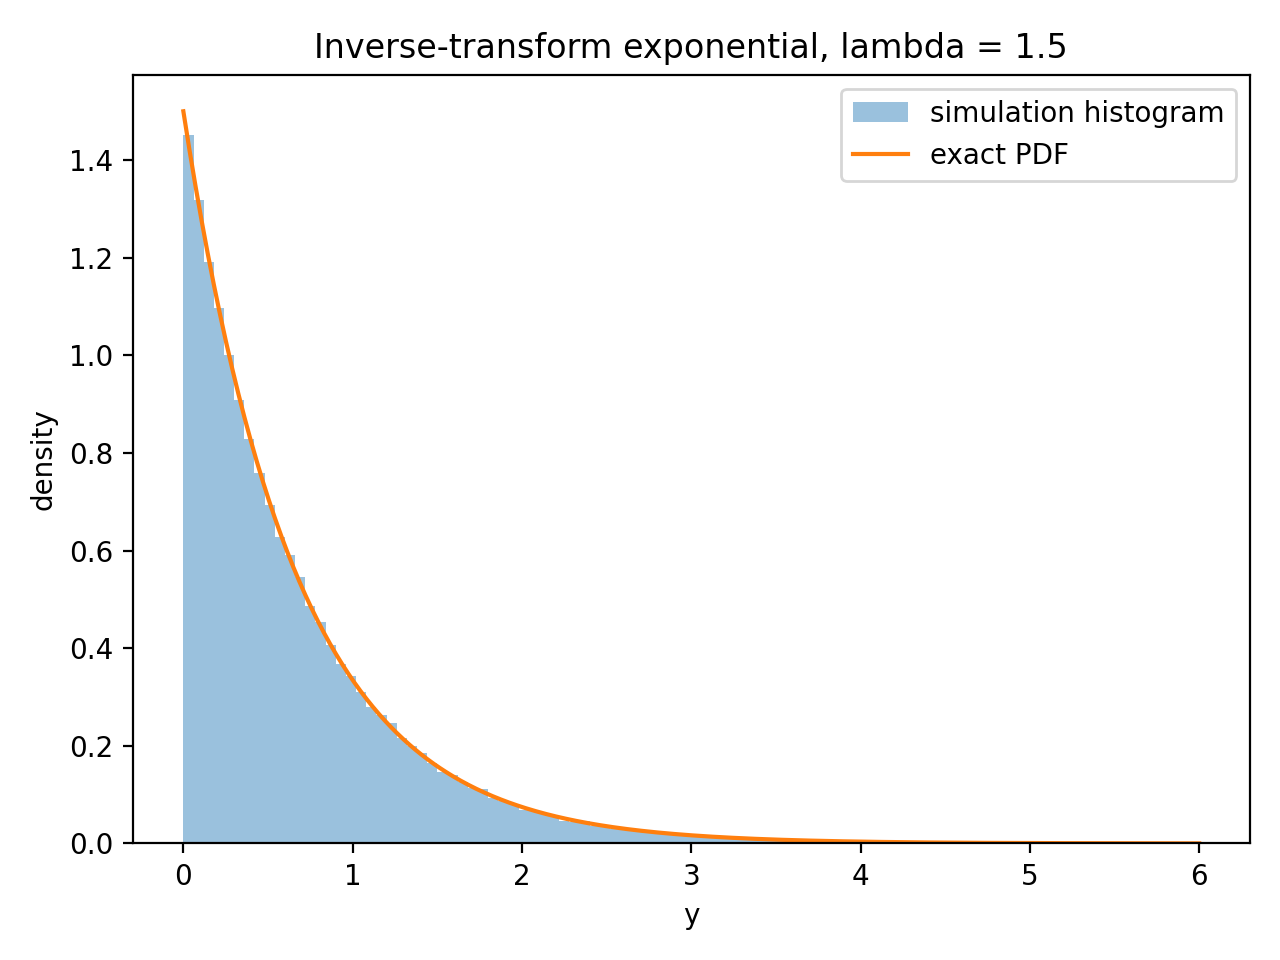
\includegraphics[width=0.78\textwidth]{ex4_exp_pdf.png}
\caption{Histogram of the simulated exponential sample compared with the exact PDF $1.5e^{-1.5y}$.}
\end{figure}

\subsection*{Numerical check}
The sample mean is
\begin{equation}
    \bar Y \approx 0.664903.
\end{equation}
The theoretical mean is
\begin{equation}
    \mathbb{E}[Y] = \frac{1}{\lambda} = \frac{1}{1.5} \approx 0.666667.
\end{equation}
The agreement is good, and the histogram follows the theoretical exponential density.

\section{Empirical CDF}

\subsection*{Method}
For a sample $Y_1,\ldots,Y_M$, the empirical cumulative distribution function is
\begin{equation}
    \hat F_M(y) = \frac{1}{M}\sum_{i=1}^M \mathbf{1}\{Y_i\leq y\}.
\end{equation}
For the exponential distribution with $\lambda=1.5$, the exact CDF is
\begin{equation}
    F_Y(y)=1-e^{-1.5y}, \qquad y\geq 0.
\end{equation}

\subsection*{Simulation result}
\begin{figure}[H]
\centering
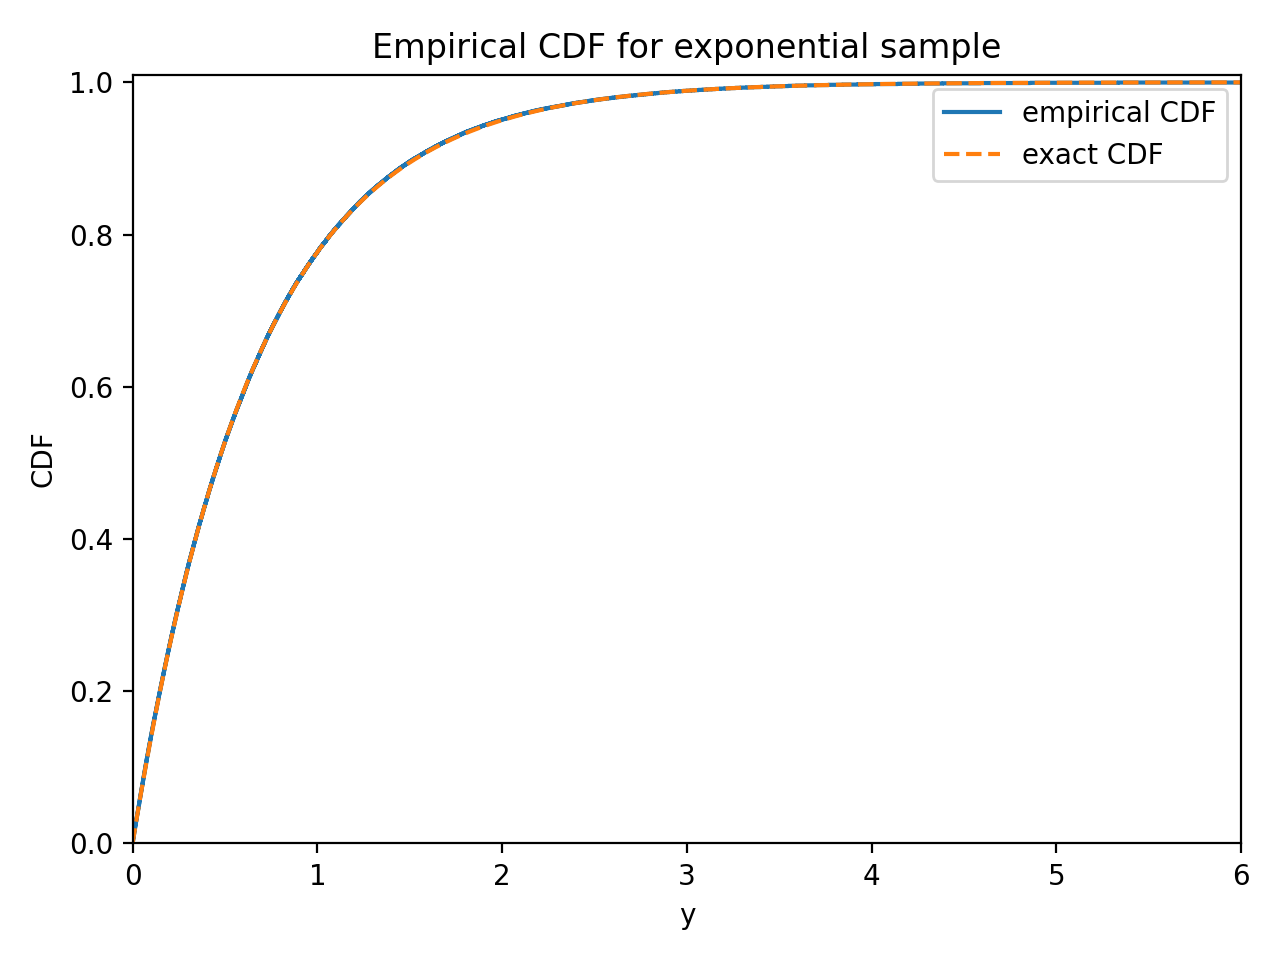
\includegraphics[width=0.78\textwidth]{ex5_exp_ecdf.png}
\caption{Empirical CDF of the exponential sample compared with the exact CDF $1-e^{-1.5y}$.}
\end{figure}

The empirical CDF is close to the theoretical CDF.  Small deviations are caused by finite-sample randomness.  As the sample size increases, the empirical CDF converges uniformly to the true CDF according to the Glivenko--Cantelli theorem.

\section*{Code}
The full Python code used to generate the results and figures is included below.

\lstinputlisting{HomeWork07_solution.py}

\end{document}
